

\فصل{مقدمه}

چهارپره یا کوادکوپتر\LTRfootnote{Quadcopter} یکی از انواع وسایل پهپاد\footnote{پرنده‌ی هدایت‌پذیر از دور} است. چهارپره‌ها نوعی هواگرد بالگردان هستند و در دسته‌ی چندپروانه‌ها جای دارند و به دلیل کمک گرفتن از چهار پروانه برای نیروی پیشرانش، به عنوان کواد (چهار) کوپتر نامیده می‌شوند. چهارپره‌ها به دلیل داشتن قدرت مانور فوق‌العاده و پروازهایی با تعادل بالا از کاربردهای بسیار گسترده‌ای برخوردارند.
در سال‌های اخیر توجه شرکت‌ها، دانشگاه‌ها و مراکز تحقیقاتی بیش از پیش به این نوع از پهپادها جلب شده‌است و لذا روزانه پیشرفت چشم‌گیری در امکانات و پرواز این نوع از پرنده‌ها مشاهده می‌کنیم. چهارپره‌ها در زمینه‌های تحقیقاتی، نظامی، تصویر برداری، تفریحی و سمپاشی از کاربرد بالا و روزافزونی برخوردارند و مدل‌های دارای سرنشین آن نیز تولید شده‌است.





\قسمت{تاریخچه}
مدل‬ اولیه آزمایشی یک چندموتوره\LTRfootnote{Multiroter} در سال ۱۹۰۷ توسط دو برادر فرانسوی بنام \lr{Jacques and Louis Breguet} در پروژه‌ای بنام Quadcopter ساخته و تست شد، هرچند آن‌ها نتوانستند پرنده خود را در آسمان نگه دارند ولی موفق به پرواز ثابت شدند. بعد از آن ساخت بالگرد چهار پروانه‌ای به سال ۱۹۲۰ میلادی برمیگرد. در آن سال یک مهندس فرانسوی بنام \lr{etienne oehmichen} اولین بالگرد چهارپره را اختراع کرد و مسافت ۳۶۰ متر را با چهارپره خود پرواز کرد. در همان سال او مسافت یک کیلومتر را در مدت هفت دقیقه و چهل ثانیه پرواز کرد.

در  سال ۱۹۲۲ در آمریکا \lr{Dr George de Btheza} موفق به ساخت و تست تعدادی چهارپره برای ارتش شد که قابلیت کنترل و حرکت در سه بعد را داشت، ولی پرواز با آن بسیار سخت بود.

در سال‌های اخیر توجه مراکز دانشگاهی به طراحی و ساخت پهپادهای چهارپره جلب شده‌است و مدل‌های مختلفی در دانشگاه استنفورد و کورنل ساخته شده است و به تدریج رواج یافته‌است~\cite{5717652}.

از حدود سال ۲۰۰۶ کواد کوپترها شروع به رشد صنعتی به صورت وسایل پرنده بدون سرنشین نمودند.


\قسمت{تعریف مسئله}
مسئله‌ای که در این پروژه بررسی می‌شود، کنترل وضعیت سه درجه آزادی استند آزمایشگاهی چهارپره با استفاده از روش کنترل خطی مربعی مبتنی بر بازی دیفرانسیلی است. این استند آزمایشگاهی شامل یک چهارپره است که از 
مرکز توسط یک اتصال به یک پایه وصل شده است. در این صورت، تنها وضعیت (زوایای رول\LTRfootnote{Roll}، پیچ\LTRfootnote{Pitch} و یاو\LTRfootnote{Yaw}) 
چهارپره تغییر کرده و فاقد حرکت انتقالی است. همچنین می‌توان با مقید کردن چرخش حول هر محور ، 
حرکات رول، پیچ و یاو  پرنده را به صورت مجزا و یا با یکدیگر بررسی کرد.
استند آزمایشگاهی سه درجه آزادی چهارپره در شکل \ref{LabQuad} نشان داده شده ‌است.

\begin{figure}[H]\label{LabQuad}
	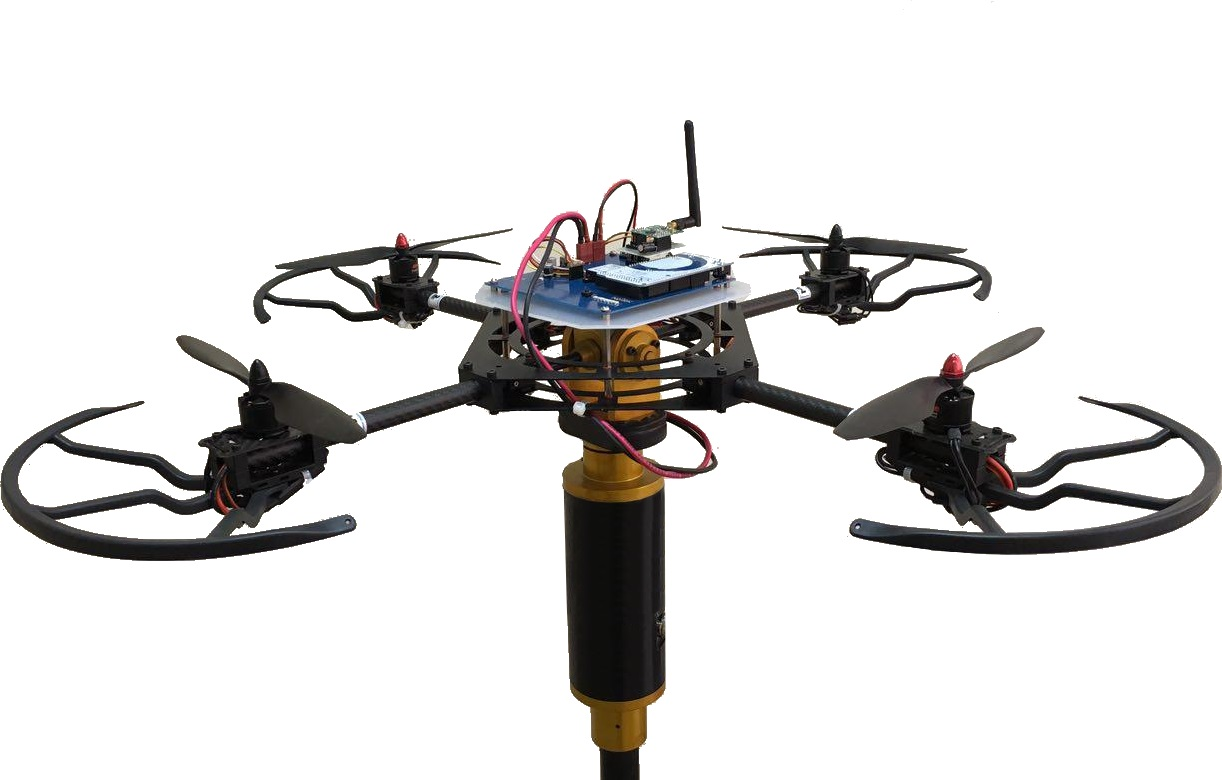
\includegraphics[width=12cm]{../../Figures/introduction/3DOFQuad.jpg}
	\centering
	\caption{استند سه درجه آزادی چهارپره آزمایشگاه 
	\cite{Iranlabexpo}}
\end{figure}
با توجه به شکل مرکز جرم این استند بالاتر از مفصل قرار دارد که می‌توان آن را به صورت آونگ معکوس در نظر گرفت. بنابراین سیستم بدون حضور کنترل کننده ناپایدار است. این سیستم دارای چهار ورودی مستقل (سرعت چرخش پره‌ها) و سه خروجی زاویه‌ای اویلر ($\psi, \theta, \phi$) است. در مدل سازی این استند عدم قطعیت وجود دارد، اما با توجه به کنترل کننده مورد استفاده می‌توان این عدم قطعیت را به صورت اغتشاش در نظر گرفت و سیستم را به خوبی کنترل کرد. در پایان این کنترل کننده با کنترل کننده تناسبی-انتگرالی-مشتقی\LTRfootnote{PID (Proportional–Integral–Derivative)} 
و کنترل کننده رگلاتور مربعی خطی\LTRfootnote{LQR (Linear Quadratic Regulator)} مقایسه خواهد ‌شد.


\subsection{ساختار بالگرد}

چهارپره‌ها همانند انواع دیگر وسایل پرنده از ایجاد اختلاف فشار در اتمسفر پیرامون خود برای بلند شدن و حرکت در هوا استفاده می‌کنند. همان‌طور که بالگردها به کمک پره اصلی این اختلاف فشار را ایجاد می‌کنند و نیروی برآی\LTRfootnote{Thrust}
 خود را تأمین می‌کنند. به دلیل وجود نیروی عمل و عکس‌العمل در بالگردها، پس از اینکه پره اصلی شروع به چرخش می‌کند با برخورد مولکول‌های هوا به این پره و وجود عکس‌العمل، یک نیرویی با جهت مخالف جهت چرخش پره به پره و در ادامه به شفت متصل به پره اعمال می‌شود (نیروی گشتاور) و این نیرو باعث چرخش بالگرد به دور خود می‌شود. حال برای حل این مشکل از پره دم بالگرد استفاده می‌شود تا نیرویی را تولید کند که مانع چرخش بالگرد به دور خود شود. حال اگر بالگرد به جای داشتن یک پره اصلی از دو پره اصلی که خلاف جهت یکدیگر بچرخند استفاده می‌نمود، به دلیل خنثی شدن دو نیروی گشتاور توسط یکدیگر، دیگر بالگرد به دور خود نمی‌چرخید. مانند بالگردهای شینوک\LTRfootnote{Boeing CH-47 Chinook} که نمایی از آن در شکل
\ref{chinook}
  آورده شده‌است. حال با توجه به توضیحات داده شده راحت‌تر می‌توان به ساختار چهارپره‌ها اشاره نمود.
\begin{figure}[H]
	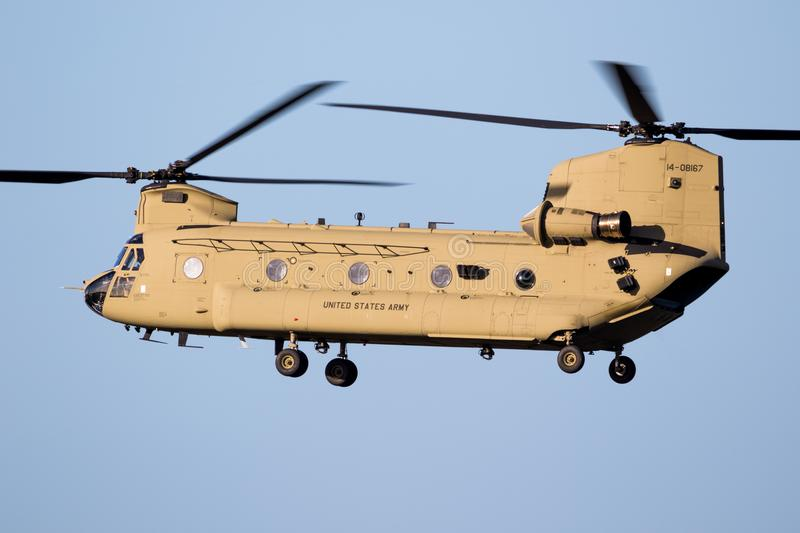
\includegraphics[width=12cm]{../../Figures/introduction/boeing-ch-chinook.jpg}
	\centering
	\caption{بالگرد شینوک
		\cite{CH-47}}
	\label{chinook}
\end{figure}
\subsection{ساختار چهارپره}


چهارپره‌ها با بهره‌گیری از چهار موتور و پره مجزا و چرخش دو به دو معکوس این موتورها نیروی گشتاورهای ایجاد شده را خنثی می‌کنند و همچنین اختلاف فشار لازم جهت ایجاد نیروی برآ را تأمین می‌کنند.

\begin{figure}[H]
	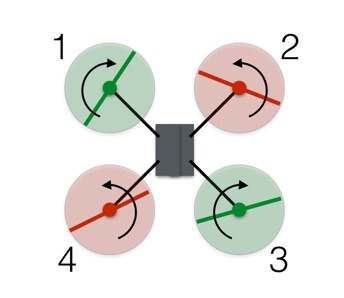
\includegraphics[width=12cm]{../../Figures/introduction/Quadblade.jpg}
	\centering
	\caption{جهت چرخش پره‌های چهارپره
		\cite{Quadhowfly}}
\end{figure}

نحوه ایجاد فرامین کنترلی در چهارپره‌ها به این صورت است که برای تغییر ارتفاع از کم یا زیاد کردن سرعت چرخش همه موتورها استفاده می‌شود و باعث کمتر یا زیاد تر شدن نیروی برآ می‌شود. برای چرخش چهارپره به دور خود و به صورت درجا، دو پره هم جهت با سرعت کمتر و دو پره هم جهت دیگر با سرعت بیشتر می‌چرخند و نیروی گشتاور به یک سمت ایجاد می‌شود و نیروی برآ همانند قبل است (زیرا دو پره با سرعت کمتر و دو پره دیگر به همان نسبت با سرعت بیشتر می‌چرخند) لذا چهارپره در ارتفاع ثابت به دور خود می‌چرخد. برای حرکت چهارپره‌ها در جهت‌های مختلف (عقب، جلو، چپ و راست) توسط کم و زیاد کردن سرعت موتورها چهارپره را از حالت افقی خارج کرده و باعث حرکت آن می‌شوند.


\section{تئوری بازی}
تئوری بازی با استفاده از مدل‌های ریاضی به تحلیل روش‌های همکاری یا رقابت موجودات منطقی و هوشمند می‌پردازد. تئوری بازی، شاخه‌ای از ریاضیات کاربردی است که در علوم اجتماعی و به ویژه در اقتصاد، زیست‌شناسی، مهندسی، علوم سیاسی، روابط بین‌الملل، علوم رایانه، بازاریابی و فلسفه مورد استفاده قرار می‌گیرد. تئوری بازی در تلاش است تا به وسیله‌ی ریاضیات، رفتار را در شرایط راهبردی یا در یک بازی که در آن‌ها موفقیت فرد در انتخاب کردن، وابسته به انتخاب دیگران می‌باشد، برآورد کند.
\subsection{تاریخچه تئوری بازی}
%در سال ۱۹۲۱ یک ریاضی‌دان فرانسوی به نام اِمیل بُرِل برای نخستین بار به مطالعهٔ تعدادی از بازی‌های رایج در قمارخانه‌ها پرداخت و چند مقاله در موردِ آن‌ها نوشت. او در این مقاله‌ها بر قابل پیش‌بینی بودنِ نتایجِ این نوع بازی‌ها از راه‌های منطقی، تأکید کرده بود. 
%کوتاه است یا نه؟؟؟؟؟؟؟؟؟؟؟
در سال ۱۹۹۴ جان فوربز نش به همراه جان هارسانی و راینهارد سیلتن به خاطر مطالعات خلاقانه خود در زمینهٔ نظریهٔ بازی، برنده‌ی جایزه نوبل اقتصاد شدند. در سال‌های پس از آن نیز بسیاری از برندگان جایزه‌ی نوبل اقتصاد از میان متخصصین تئوری بازی انتخاب شدند. آخرین آنها، ژان تیرول فرانسوی است که در سال ۲۰۱۴ این جایزه را کسب کرد \cite{nobel}.
\subsection{تعادل نش}
پژوهش‌ها در این زمینه اغلب بر مجموعه‌ای از راهبردهای شناخته شده به عنوان تعادل در بازی‌ها استوار است. این راهبردها اصولاً از قواعد عقلانی به نتیجه می‌رسند. مشهورترین تعادل‌ها، تعادل نش است. در تئوری بازی، تعادل نش (به نام جان فوربز نش، که آن را پیشنهاد کرد) راه حلی از تئوری بازی است که شامل دو یا چند بازیکن است، که در آن فرض بر آگاهی هر بازیکن به راهبرد تعادل دیگر بازیکنان است. بر اساس نظریهٔ تعادل نش، اگر فرض کنیم در هر بازی با استراتژی مختلط، بازیکنان به طریق منطقی و معقول راهبردهای خود را انتخاب کنند و به دنبال حد اکثر سود در بازی هستند، دست کم یک راهبرد برای به دست آوردن بهترین نتیجه برای هر بازیکن قابل انتخاب است و چنانچه بازیکن راهکار دیگری به غیر از آن را انتخاب کند، نتیجهٔ بهتری به دست نخواهد آورد.



